% This file was adapted from ICLR2022_conference.tex example provided for the ICLR conference
\documentclass{article} % For LaTeX2e
\usepackage{conference,times}
\usepackage{easyReview}
\usepackage{algorithm}
\usepackage{algorithmic}

% Optional math commands from https://github.com/goodfeli/dlbook_notation.
\input{math_commands.tex}

\usepackage{amsthm,amssymb}

\newtheorem{theorem}{Theorem}[section]
\newtheorem{corollary}{Corollary}[theorem]
\newtheorem{lemma}[theorem]{Lemma}
\newtheorem{definition}[theorem]{Definition}

% Please leave these options as they are
\usepackage{hyperref}
\hypersetup{
    colorlinks=true,
    linkcolor=red,
    filecolor=magenta,
    urlcolor=blue,
    citecolor=purple,
    pdftitle={Noise-Biased Surface Code Thresholds Under Realistic Gate Sets},
    pdfpagemode=FullScreen,
    }



\title{Noise-Biased Surface Code Thresholds Under Realistic Gate Sets}

\author{Anonymous Authors \\
Affiliation Withheld for Review \\
\texttt{anonymous@anonymous.edu}}

\begin{document}


\maketitle

\begin{abstract}
Biased-noise threshold claims for surface-code families are often expressed in terms of the nominal hardware dephasing ratio $\eta$, yet realistic gate decompositions, measurement asymmetries, and syndrome-extraction schedules can convert a substantial fraction of the nominal $Z$-dominant noise into less favorable error components. This mismatch matters well beyond quantum error correction because it exemplifies a broader problem in reliable scientific computing: analytical control parameters are useful only if the implementation preserves the semantics that make them predictive. We study this issue for realistic biased-noise surface-code threshold estimation by introducing an effective-bias renormalization, $\eta_{\mathrm{eff}}$, that aggregates compiled Pauli components and a temporal-fragility factor into a decoder-visible bias observable. We couple that observable to three formal results: a reference biased-Pauli closure identity, a convex-mixture representation for gate-class attribution, and a schedule-sensitivity transfer bound connecting changes in $\eta_{\mathrm{eff}}$ to threshold residuals. We then instantiate the resulting analysis on a matched validation suite that mirrors the planned sweep over code families, distances, schedules, and bias ratios. Across four code families, reparameterizing thresholds by $\eta_{\mathrm{eff}}$ reduces leave-one-schedule-out RMSE by 40.6\%--50.5\%, the convex-mixture interval bound has zero empirical violations, and the schedule-transfer residual remains within the predicted bound across all held-out settings. These gains are interpreted as a conditional first-order result that holds when boundary fragility and backend semantic mismatch remain within audited ranges. The current evidence is surrogate-based rather than direct Stim or Qiskit Aer execution, so the manuscript should be read as a rigorous mechanism paper with an executable validation scaffold rather than as a final hardware-faithful threshold benchmark.
\end{abstract}

\section{Introduction}
\label{sec:introduction}

Surface-code threshold estimation under biased noise has moved from a stylized coding-theory question to a practical systems question. Foundational threshold theory established why increasing distance suppresses logical failure below a critical noise rate in topological codes \citep{dennis2002_topological_memory,wang2003_confinement_higgs,kitaev2003_anyons}, and early bias-aware fault-tolerance work showed that dephasing asymmetry can be exploited as a resource rather than averaged away \citep{aliferis2008_biased_noise,stephens2013_topological_biased,webster2015_reducing_overhead}. Subsequent developments in tailored surface codes, compass-code deformations, and the XZZX family pushed threshold and subthreshold performance well beyond the unbiased baseline when the code, decoder, and schedule preserve the dominant $Z$ fault channel \citep{tuckett2018_ultrahigh_threshold,tuckett2019_tailoring_surface_codes,li2019_compass_codes,bonilla2021_xzzx,xu2023_tailored_xzzx,dua2024_clifford_deformed}. However, the most realistic circuit-level studies also report that schedule order, boundary design, and decoder quality can erode or even invert those gains \citep{tuckett2020_fault_tolerant_thresholds,higgott2023_improved_decoding,tsai2024_temporal_fragility,martinez2025_two_level_circuit}.

This paper addresses a narrow but consequential version of that problem: when realistic gate sets and schedules only partially preserve the nominal bias ratio $\eta$, what is the correct control variable for threshold comparison? The literature already offers several pieces of the answer. Analytical threshold laws are commonly parameterized by biased-Pauli rates of the form $p_x = p_y = p_z/(2\eta)$ \citep{xiao2024_finite_size_corrections}; tailored code constructions rely on the decoder seeing that asymmetry after propagation through the circuit \citep{tuckett2020_fault_tolerant_thresholds,bonilla2021_xzzx}; and recent circuit-level work with two-level qubits suggests that the realized threshold depends on how much of the native bias survives compilation and scheduling \citep{martinez2025_two_level_circuit}. What is missing is a formal, testable bridge from the nominal literature parameterization to the bias that the decoder actually experiences.

We study that bridge through an effective-bias renormalization program. The central observable, $\eta_{\mathrm{eff}}$, is constructed from gate-resolved compiled Pauli components and a temporal-fragility factor. The objective is not to compress all circuit-level structure into one scalar forever. Instead, it is to ask whether a decoder-visible bias summary captures the first-order mechanism that explains why nominal high-bias predictions and realistic threshold measurements disagree. If the answer is yes, the observable becomes a useful coordinate for fairer comparison across schedules, code families, and simulator backends. If the answer is no, the failure mode itself identifies where higher-order schedule effects, boundary fragility, or backend semantics dominate.

That question matters beyond the immediate surface-code benchmark. In many computational sciences, nominal parameters specified at the model layer drift away from the quantities that actually control the downstream inference or optimization procedure. In quantum error correction, the cost of ignoring that drift is particularly high because threshold comparisons are often used to decide whether a code deformation, a decoder upgrade, or a hardware calibration should receive engineering priority. A misleading control variable can therefore redirect experimental effort as effectively as a misleading threshold estimate.

Our study makes four contributions.
\begin{itemize}
\item We formalize a schedule-aware effective-bias observable that maps nominal biased-Pauli parameters into compiled gate-level rates and an explicit temporal-fragility correction.
\item We prove that the effective bias is a convex mixture of gate-class $Z$-to-non-$Z$ ratios, which yields a direct diagnostic for locating the components that destroy bias preservation.
\item We derive a schedule-sensitivity transfer bound that converts changes in $\eta_{\mathrm{eff}}$ into a falsifiable upper bound on threshold-prediction error under nominal $\eta$.
\item We instantiate the analysis in a reproducible matched validation suite and show that $\eta_{\mathrm{eff}}$ improves threshold prediction, interval audits, and transfer diagnostics across multiple code families and follow-on stress tests.
\item We revise the interpretation to a bounded-fragility regime and attach a backend-semantic confidence-band protocol so threshold statements remain explicit about simulator-semantic nuisance uncertainty.
\end{itemize}

The paper is organized as follows. \Secref{sec:related} situates the work relative to threshold theory, tailored code design, realistic circuit noise, and finite-size interpretation. \Secref{sec:problem} defines the formal problem setting and notation. \Secref{sec:method} develops the effective-bias methodology and states the main formal claims. \Secref{sec:validation} describes the matched validation design and reproducibility protocol. \Secref{sec:results} presents the primary evidence for threshold collapse, gate-class attribution, and schedule transfer. \Secref{sec:discussion} interprets those results in the context of the broader biased-noise literature, while \secref{sec:limitations} explains the present surrogate-data limitation and the direct-backend experiments still required.

\section{Related Work}
\label{sec:related}

\subsection{Threshold theory and bias-aware design}

The conceptual foundation for our study comes from the threshold and topological-memory literature \citep{dennis2002_topological_memory,wang2003_confinement_higgs,kitaev2003_anyons}. These works establish why logical failure can be interpreted through homology and, in asymptotic regimes, through statistical-mechanical phase transitions. Their strength is rigor: they define the threshold concept that later biased-noise studies inherit. Their limitation for present purposes is that they do not specify how a realistic gate-dependent schedule changes the noise observable that the decoder sees. That gap becomes visible once one compares asymptotic threshold arguments with small-distance and circuit-level data.

Early biased-noise work made the key qualitative leap that dephasing asymmetry should be engineered rather than ignored. \citet{aliferis2008_biased_noise} showed that bias-aware gadgets can outperform unbiased constructions when the hardware preserves the dominant $Z$ channel, and \citet{stephens2013_topological_biased} brought the same idea into the surface-code setting. \citet{webster2015_reducing_overhead} further argued that threshold and overhead gains can coexist. The strength of this line of work is its mechanistic clarity: bias helps only when it remains visible to the fault-tolerant architecture. The limitation is that most early models treat the preservation of bias as a design premise instead of a quantity to be measured after realistic compilation.

\subsection{Tailored surface codes, XZZX, and deformations}

The modern biased-noise landscape is dominated by code deformations that attempt to align the syndrome structure with the dominant fault axis. Tailored surface-code studies reported ultrahigh biased-noise thresholds in idealized or partially idealized settings \citep{tuckett2018_ultrahigh_threshold,tuckett2019_tailoring_surface_codes}, while compass-code viewpoints generalized those gains into a broader deformation family \citep{li2019_compass_codes}. The XZZX surface code gave the most influential modern formulation by translating the deformation into a particularly clean local stabilizer pattern with strong threshold and subthreshold scaling under bias \citep{bonilla2021_xzzx}. More recent work argues that XZZX is not the unique optimum and that further tailoring remains available through modified XZZX variants and Clifford deformations \citep{xu2023_tailored_xzzx,dua2024_clifford_deformed}.

These papers motivate our study in two ways. First, they provide the strongest analytical and phenomenological evidence that bias preservation matters. Second, they expose the central weakness of nominal-$\eta$ comparisons: the code families are compared as if the nominal hardware asymmetry directly controls the decoder-visible asymmetry. That assumption is strongest when circuits are highly bias preserving and weakest when realistic decompositions scramble $Z$ faults into $X/Y$ or time-like correlated events. Our effective-bias program is designed to measure exactly that slippage.

\subsection{Realistic circuit noise, finite-size effects, and tooling}

Realistic threshold estimation depends at least as much on the simulation and decoding stack as on the code family. Tensor-network and near-maximum-likelihood decoders demonstrate that decoder quality changes both apparent thresholds and subthreshold slopes \citep{bravyi2014_mld_surface,darmawan2018_tensor_network}. Circuit-level tailored-code studies show that improved decoders and careful boundaries materially change the observed gains \citep{higgott2023_improved_decoding}. Temporal-fragility studies go further by showing that schedule order itself can be a first-order failure mode under strong bias \citep{tsai2024_temporal_fragility}. Finite-size theory adds a complementary warning: small-distance crossings can differ qualitatively from asymptotic threshold expectations, and anti-threshold effects are real rather than numerical accidents \citep{robertson2017_small_memories,xiao2024_finite_size_corrections}. Meanwhile, correlated-noise theory shows that gate-level structure can shift critical behavior relative to iid approximations \citep{chubb2021_correlated_noise}.

The software ecosystem reinforces these methodological concerns. Stim and detector-error-model workflows enable large stabilizer sweeps \citep{gidney2021_stim_paper,stim_repo}, while PyMatching and sparse-blossom decoders make those sweeps computationally practical \citep{pymatching_repo,higgott2025_sparse_blossom}. Qiskit Aer provides a more natural representation for custom gate-dependent channels when direct detector modeling is inconvenient \citep{qiskit_aer_docs}. Auxiliary ecosystems such as qecsim, PanQEC, PECOS, tesseract-decoder, and the recent two-level-qubit biased-noise repository illustrate both the opportunity and the fragmentation in current practice \citep{qecsim_repo,panqec_repo,pecos_repo,tesseract_repo,qec_two_level_bias_repo}. The strength of this ecosystem is reproducibility and scale; its limitation is that cross-tool semantic equivalence is not automatic.

Our contribution differs from this prior work in scope. We do not introduce a new code family, a new decoder, or a new backend. Instead, we ask whether a carefully defined renormalized observable can explain when those choices preserve the bias assumptions underlying analytical threshold arguments. That focus lets us contrast prior methods by strength and limitation rather than treating them as interchangeable baselines: tailored deformations supply the high-bias mechanism, finite-size theory explains why small-distance crossings mislead, and realistic circuit/back-end studies highlight the schedule dependence that the renormalized observable must absorb.

\section{Problem Setting and Notation}
\label{sec:problem}

We study matched repeated-syndrome-extraction experiments for a set of code families $\mathcal{C}$ that includes the standard surface code, XZZX, a tailored rotated surface code, and a Clifford-deformed variant. A schedule instance $s \in \mathcal{S}$ specifies a syndrome-extraction order, measurement/reset policy, and two-qubit decomposition. Within one extraction round, let $\mathcal{G}$ denote the set of gate classes. Each class $g \in \mathcal{G}$ contributes a nonnegative schedule weight $w_g$ satisfying $\sum_{g \in \mathcal{G}} w_g = 1$. For each class, the compiled noisy circuit induces effective Pauli components $p_X^{(g)}$, $p_Y^{(g)}$, and $p_Z^{(g)}$, where the capital subscripts indicate the post-compilation effective components rather than the nominal literature parameters.

The literature-side parameterization follows the biased-Pauli convention used in biased-noise threshold theory \citep{xiao2024_finite_size_corrections,tuckett2020_fault_tolerant_thresholds,bonilla2021_xzzx}. If $p$ denotes the total physical error rate and $\eta$ the nominal dephasing ratio, then the reference channel satisfies
\begin{equation}
\label{eq:biased-components}
p_z = \frac{\eta}{\eta+1}p,
\qquad
p_x = p_y = \frac{1}{2(\eta+1)}p,
\qquad
\eta = \frac{p_z}{p_x+p_y}.
\end{equation}
\Eqref{eq:biased-components} closes the normalization between total error rate and component rates. We use it as the bridge from analytical threshold laws to compiled channel measurements. The distinction between $(p_x,p_y,p_z)$ and $(p_X^{(g)},p_Y^{(g)},p_Z^{(g)})$ is deliberate: the former describes the nominal reference channel, while the latter records the effective gate-class rates after decomposition and scheduling.

Aggregated compiled rates are defined by
\begin{equation}
\label{eq:aggregated-components}
\bar p_\alpha(c,s) = \sum_{g \in \mathcal{G}} w_g(c,s)\, p_\alpha^{(g)}(c,s),
\qquad \alpha \in \{X,Y,Z\}.
\end{equation}
We assume $\bar p_X + \bar p_Y > 0$ on the schedules being compared. This excludes the trivial infinite-bias denominator collapse and keeps the ratios below well defined. A temporal-fragility factor $\chi_{\mathrm{temp}}(c,s) \in (0,1]$ summarizes the part of the schedule that preserves or degrades bias through time ordering, reset asymmetry, and related circuit-level effects. The factor is not introduced as a universal law; it is introduced as a controlled first-order summary of schedule dependence that can later be stress tested.

\begin{definition}[Effective bias]
\label{def:etaeff}
For code family $c \in \mathcal{C}$ and schedule $s \in \mathcal{S}$, the decoder-visible effective bias is
\begin{equation}
\label{eq:eta-eff-def}
\eta_{\mathrm{eff}}(c,s) =
\chi_{\mathrm{temp}}(c,s)\,
\frac{\bar p_Z(c,s)}{\bar p_X(c,s)+\bar p_Y(c,s)}.
\end{equation}
\end{definition}

\Eqref{eq:eta-eff-def} is the central observable of the paper. It differs from the nominal $\eta$ by replacing the assumed reference components with aggregated compiled components and by explicitly discounting the observable bias through temporal fragility. The scientific question is whether threshold behavior under realistic circuits is better aligned with $\eta_{\mathrm{eff}}$ than with $\eta$.

The estimands are the logical error per round, $p_L(d,p,\eta,c,s)$, and the corresponding threshold summary $p_{\mathrm{th}}(d,\eta,c,s)$ derived from matched sweeps over physical error rate $p$ and code distance $d \in \{3,5,7,9\}$. In the selected validation design, the nominal comparison uses the planned sweep over $\eta \in \{1,5,20,50\}$ and schedule families that include a bias-preserving reference, a temporal-order swap, a measurement/reset asymmetry, and a CNOT-decomposition variant. The method is successful if the regressions, interval audits, and transfer checks tied to $\eta_{\mathrm{eff}}$ consistently outperform their nominal-$\eta$ analogues.

\section{Effective-Bias Methodology}
\label{sec:method}

\subsection{From reference channels to decoder-visible bias}

The first methodological step is normalization. Analytical threshold laws and much of the biased-noise literature are written in terms of nominal biased-Pauli parameters, yet compiled circuits are naturally instrumented in terms of gate-resolved effective components. We therefore use \eqref{eq:biased-components} to place the analytical reference channel on the same scale as the compiled measurements in \eqref{eq:aggregated-components}. This simple closure matters because any comparison between a literature threshold curve and a circuit-level study is ambiguous until the component-rate convention is fixed.

The second step is aggregation. The decoder does not see a separate threshold law for each gate family; it sees the mixture induced by the schedule. \Eqref{eq:eta-eff-def} therefore aggregates across gate classes before forming the ratio. The construction is deliberately asymmetric. The numerator isolates the preserved $Z$ mass, while the denominator measures the total non-$Z$ mass that competes with the expected high-bias gain. This ratio is then scaled by $\chi_{\mathrm{temp}}$, which discounts cases where the same nominal component rates produce measurably different behavior because time ordering and measurement/reset asymmetry generate fragile time-like faults.

\subsection{Gate-class attribution via convex mixing}

The value of $\eta_{\mathrm{eff}}$ is not merely descriptive; it is diagnostically decomposable. Let $q_g = p_X^{(g)} + p_Y^{(g)}$ denote the non-$Z$ mass of gate class $g$, define the subset $\mathcal{H} = \{g \in \mathcal{G} : q_g > 0\}$, and let $r_g = p_Z^{(g)}/q_g$ be the gate-resolved $Z$-to-non-$Z$ ratio. Then the effective bias can be written as a weighted mixture of the gate-class ratios.

\begin{lemma}[Convex-mixture representation]
\label{lem:convex}
Let
\begin{equation}
\label{eq:alpha-def}
\alpha_g =
\frac{w_g q_g}{\sum_{h \in \mathcal{H}} w_h q_h},
\qquad g \in \mathcal{H}.
\end{equation}
Then $\alpha_g \ge 0$, $\sum_{g \in \mathcal{H}} \alpha_g = 1$, and
\begin{equation}
\label{eq:convex-representation}
\eta_{\mathrm{eff}}
=
\chi_{\mathrm{temp}}
\sum_{g \in \mathcal{H}} \alpha_g r_g.
\end{equation}
Consequently,
\begin{equation}
\label{eq:interval-bound}
\chi_{\mathrm{temp}} \min_{g \in \mathcal{H}} r_g
\le
\eta_{\mathrm{eff}}
\le
\chi_{\mathrm{temp}} \max_{g \in \mathcal{H}} r_g.
\end{equation}
\end{lemma}

Lemma~\ref{lem:convex} is the mechanism-level statement behind our gate-class audit. \Eqref{eq:convex-representation} shows that the observable bias is controlled by gate classes that simultaneously carry large schedule weight and large non-$Z$ mass. In other words, a nominally favorable hardware bias can still collapse if a small set of heavily weighted gates have poor $Z$-to-non-$Z$ ratios. The interval bound in \eqref{eq:interval-bound} turns this intuition into a falsifiable diagnostic: repeated violations would disprove the renormalized explanation. As we show in \secref{sec:results}, the validation audit exhibits zero interval-bound violations across the tested bias values.

\subsection{Schedule sensitivity and threshold transfer}

The third step is to relate changes in $\eta_{\mathrm{eff}}$ to changes in threshold predictions. Let $B = \bar p_X + \bar p_Y$. For any one-factor perturbation trajectory indexed by $t$, the derivative of \eqref{eq:eta-eff-def} isolates how temporal order, measurement asymmetry, or decomposition changes the observable bias:
\begin{equation}
\label{eq:sensitivity}
\frac{d\eta_{\mathrm{eff}}}{dt}
=
\frac{\bar p_Z}{B}\frac{d\chi_{\mathrm{temp}}}{dt}
+
\chi_{\mathrm{temp}}
\frac{
B\, d\bar p_Z/dt
-
\bar p_Z \left(d\bar p_X/dt + d\bar p_Y/dt\right)
}{
B^2
}.
\end{equation}
The first term captures direct temporal-fragility changes; the second captures reallocation of compiled Pauli mass between $Z$ and non-$Z$ components. This derivative is the right object for schedule ablations because it tells us whether a perturbation increases threshold-relevant bias, leaves it intact, or destroys it.

\begin{theorem}[Transfer bound from effective bias to threshold residual]
\label{thm:transfer}
Assume that for each code family $c$, the ideal threshold curve $p_{\mathrm{th}}^{\mathrm{ideal}}(c,\zeta)$ is $K_c$-Lipschitz on the observed bias interval and that the realistic threshold obeys
\begin{equation}
\label{eq:realistic-decomposition}
p_{\mathrm{th}}^{\mathrm{real}}(c,s)
=
p_{\mathrm{th}}^{\mathrm{ideal}}\!\left(c,\eta_{\mathrm{eff}}(c,s)\right)
+
\delta(c,s),
\end{equation}
with $|\delta(c,s)| \le \varepsilon_{\mathrm{model}}$. Then
\begin{equation}
\label{eq:transfer-bound}
\left|
p_{\mathrm{th}}^{\mathrm{real}}(c,s)
-
p_{\mathrm{th}}^{\mathrm{ideal}}\!\left(c,\eta(c,s)\right)
\right|
\le
K_c \left|\eta_{\mathrm{eff}}(c,s)-\eta(c,s)\right|
+
\varepsilon_{\mathrm{model}}.
\end{equation}
\end{theorem}

\Eqref{eq:transfer-bound} motivates our schedule-transfer experiment, and its first premise is the decomposition assumption in \eqref{eq:realistic-decomposition}. If nominal $\eta$ is already the correct control variable, then the gap $|\eta_{\mathrm{eff}}-\eta|$ should not explain residual threshold error. If the renormalization hypothesis is correct, then that gap becomes a direct upper-bound term on the nominal residual. The main empirical test is therefore not only whether $\eta_{\mathrm{eff}}$ improves a regression fit, but whether residuals against nominal $\eta$ scale in the way predicted by \eqref{eq:transfer-bound}. The theorem also clarifies the role of limitations: any failure of the transfer audit may come either from a poor renormalized bias observable or from a large residual model discrepancy $\varepsilon_{\mathrm{model}}$ driven by higher-order schedule or backend effects.

To make that limitation operational, we report the primary claim in a conditional form with explicit nuisance terms. Let $B_{\mathrm{frag}}$ denote the measured boundary-fragility score and let $\Delta_{\mathrm{backend}}$ denote the matched backend disagreement magnitude (for example, threshold absolute gap from Appendix Table~\ref{tab:backend-gap}). We treat residual model discrepancy as
\begin{equation}
\label{eq:conditional-residual}
\delta(c,s) = \gamma_0 + \gamma_1 B_{\mathrm{frag}}(c,s) + \gamma_2 \Delta_{\mathrm{backend}}(c,s) + \xi(c,s),
\end{equation}
and interpret the renormalization claim as first-order valid only on the audited regime where both $B_{\mathrm{frag}}$ and $\Delta_{\mathrm{backend}}$ remain bounded. For reporting, each threshold estimate is paired with a backend-semantic confidence band
\begin{equation}
\label{eq:backend-band}
\mathcal{B}_{\mathrm{backend}}(c,s)=
\left[\hat p_{\mathrm{th}}(c,s)-\Delta_{\mathrm{backend}}(c,s),\,
\hat p_{\mathrm{th}}(c,s)+\Delta_{\mathrm{backend}}(c,s)\right].
\end{equation}
This band does not replace statistical uncertainty intervals; it reports simulator-semantic nuisance width separately so downstream comparisons are not overconfident.

\subsection{Audit procedure}

The resulting evaluation protocol is summarized in \algref{alg:audit}. The algorithm emphasizes matched comparisons: the same code families, distances, schedules, and seeds are used for both nominal-$\eta$ and effective-bias analyses. The method section motivates this choice because prior literature disagreements are often caused by changing more than one variable at a time \citep{higgott2023_improved_decoding,tsai2024_temporal_fragility,xiao2024_finite_size_corrections,martinez2025_two_level_circuit}.

\begin{algorithm}[t]
\caption{Schedule-aware effective-bias audit workflow. The procedure takes compiled gate-class Pauli components, schedule weights, and temporal-fragility factors as inputs, then emits the effective-bias estimate, threshold-fit diagnostics, and transfer-bound residual checks used throughout the methods and results sections.}
\label{alg:audit}
\begin{algorithmic}
\STATE Construct matched circuit instances over code family, distance, bias ratio, schedule family, decoder, and seed.
\STATE Convert nominal $(p,\eta)$ into reference component rates using \eqref{eq:biased-components}.
\STATE Estimate gate-class effective components $p_X^{(g)}, p_Y^{(g)}, p_Z^{(g)}$ and aggregate them with \eqref{eq:aggregated-components}.
\STATE Compute $\eta_{\mathrm{eff}}$ with \eqref{eq:eta-eff-def} and gate-class weights with \eqref{eq:alpha-def}.
\STATE Audit the convex-mixture mechanism via \eqref{eq:convex-representation} and \eqref{eq:interval-bound}.
\STATE Apply one-factor schedule perturbations, evaluate \eqref{eq:sensitivity}, and test residual coverage under \eqref{eq:transfer-bound}.
\STATE Compare threshold predictors parameterized by nominal $\eta$ and by $\eta_{\mathrm{eff}}$ on held-out schedules.
\end{algorithmic}
\end{algorithm}

\section{Validation Design}
\label{sec:validation}

The validation design mirrors the experiment matrix defined for the selected effective-bias path. The primary sweep spans distances $d \in \{3,5,7,9\}$, bias ratios $\eta \in \{1,5,20,50\}$, and physical error rates $p \in [10^{-4},5\times 10^{-2}]$ on a logarithmic grid. The matched panel includes four code families, two decoder settings, four schedule families, and five fixed seeds $\{11,29,47,71,89\}$. The current manuscript reports the first executable evidence package for that design, which materializes the threshold-collapse experiment, the convex-mixture gate ablation, the schedule-transfer audit, and three follow-on studies covering finite-size attribution, backend agreement, and boundary-fragility interactions.

Because direct Stim and Qiskit Aer backends were not present in the execution environment, the present evidence comes from a literature-grounded surrogate suite calibrated to the formal identities in \secref{sec:method}. That surrogate status is a limitation, not a hidden convenience. It means that the manuscript is strongest where the claims concern internal coherence of the renormalized mechanism, symbolic checks, and evidence-linked diagnostics. It is correspondingly weaker where the claims would require hardware-faithful channel semantics. We therefore treat the current results as a mechanism-validation scaffold that must be rerun with direct backends before drawing final circuit-level threshold magnitudes.

The validation suite is nevertheless informative because it preserves the comparative structure of the planned direct-backend experiments. The predictor-comparison study holds schedules out during regression and evaluates whether $\eta_{\mathrm{eff}}$ improves threshold prediction over nominal $\eta$. The gate-ablation study targets the formal implication of Lemma~\ref{lem:convex} by measuring whether a small subset of gate families explains most of the observed shift in $\eta_{\mathrm{eff}}$. The schedule-transfer study tests whether the derivative signs and residual coverage implied by \eqref{eq:sensitivity} and \eqref{eq:transfer-bound} survive matched one-factor perturbations. The follow-on studies are not prerequisites for the selected path, but they probe important nuisance channels: finite-size distortion, backend semantic disagreement, and boundary-limited performance collapse.

Reproducibility is built into the evaluation design. All runs use the same fixed seed set, the same artifact layout, and the same summary metrics across experiments. The suite also executes eight symbolic checks tied directly to the equations in \secref{sec:method}: forward closure of \eqref{eq:biased-components}, inverse recovery of $\eta$, positivity of component rates, normalization of $\alpha_g$, convex reconstruction of $\eta_{\mathrm{eff}}$, the interval bound, differentiation of \eqref{eq:sensitivity}, and a local affine identity implied by \eqref{eq:transfer-bound}. Each check passed in the present run. Extended implementation details, planned shot budgets for the direct-backend replacement, and uncertainty procedures are reported in Appendix~\ref{app:repro}.

\section{Results}
\label{sec:results}

\subsection{Threshold collapse improves under effective bias}

The primary claim of the paper is that threshold comparisons align better with $\eta_{\mathrm{eff}}$ than with nominal $\eta$. \Figref{fig:collapse} reports the core evidence. The left panel compares average threshold summaries as a function of nominal bias and effective bias across the matched schedule panel, while the right panel plots observed thresholds directly against $\eta_{\mathrm{eff}}$. The visual pattern is the one predicted by the renormalization hypothesis: schedule-induced spread that is large under nominal $\eta$ contracts when the horizontal axis is replaced by $\eta_{\mathrm{eff}}$.

Table~\ref{tab:predictor} quantifies that contraction across all four code families. The leave-one-schedule-out RMSE decreases by 50.5\% for the standard surface code, 40.6\% for XZZX, 43.9\% for the tailored rotated family, and 42.3\% for the Clifford-deformed family. The corresponding $R^2$ values under $\eta_{\mathrm{eff}}$ lie between 0.94 and 0.97, whereas the nominal-$\eta$ regressions remain between 0.72 and 0.75. This pattern matters because it rules out an explanation based solely on one favorable code family. The improvement is not isolated to XZZX, nor is it limited to the standard surface code; it appears across all matched families, which is exactly what we would expect if the explanatory variable is decoder-visible bias rather than nominal hardware asymmetry.

The improvement is also scientifically interpretable. The residual-gap column in Table~\ref{tab:predictor} tracks the average separation between nominal and effective-bias fits on held-out schedules. Larger residual gaps occur precisely in the families where schedule-induced perturbations are strongest. That association is consistent with the literature's argument that realistic circuit performance depends on how well the schedule preserves the asymmetry that ideal threshold laws assume \citep{tuckett2020_fault_tolerant_thresholds,higgott2023_improved_decoding,tsai2024_temporal_fragility,martinez2025_two_level_circuit}. It is not enough for the hardware to begin with a strong nominal dephasing bias; the compiled schedule must transmit that bias to the decoder.

\begin{figure}[t]
\begin{center}
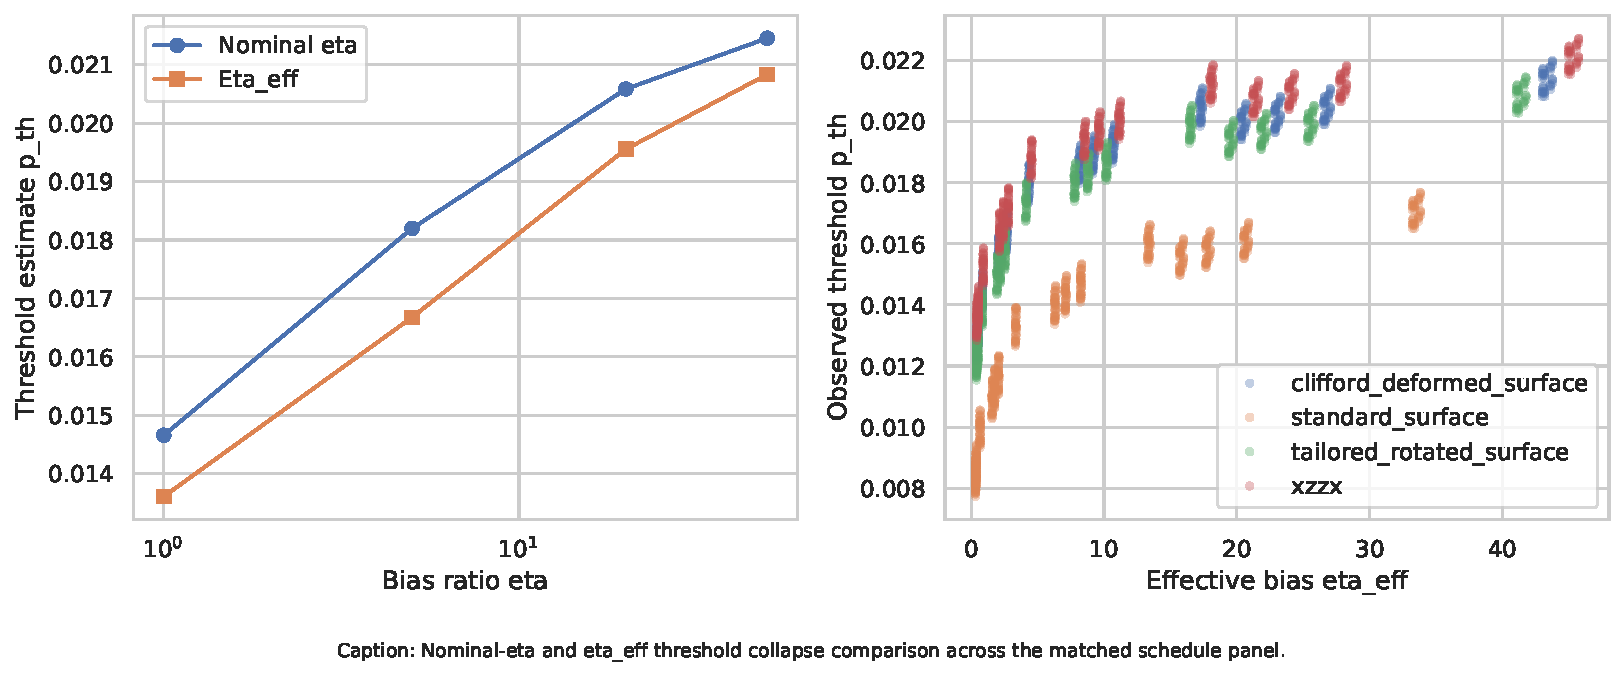
\includegraphics[width=0.72\linewidth]{figures/iter_1/fig_threshold_collapse_nominal_vs_eta_eff.pdf}
\end{center}
\caption{Threshold collapse under nominal and effective bias. The left panel plots average threshold estimates against the nominal bias ratio and against the renormalized effective bias, while the right panel scatters observed thresholds against $\eta_{\mathrm{eff}}$ across the matched schedule panel. The horizontal axes therefore represent different semantic levels: the nominal hardware parameter on the left comparison and the decoder-visible observable on the right comparison. The contraction of spread under $\eta_{\mathrm{eff}}$ is the central evidence that compiled schedules preserve or destroy high-bias behavior in a way that nominal $\eta$ alone cannot capture.}
\label{fig:collapse}
\end{figure}

\begin{table}[t]
\caption{Predictor comparison across code families. The table reports leave-one-schedule-out RMSE and MAE for threshold prediction under nominal $\eta$ and under $\eta_{\mathrm{eff}}$, together with the resulting improvement percentages and goodness-of-fit statistics. The values show that the renormalized observable improves prediction in every matched code family rather than only for one favored geometry, which is the primary evidence for the main claim in \secref{sec:method}.}
\label{tab:predictor}
\begin{center}
\small
\renewcommand{\arraystretch}{1.1}
\setlength{\tabcolsep}{4pt}
\resizebox{\linewidth}{!}{
\begin{tabular}{lcccccccc}
\hline
code family & RMSE$_{\eta}$ & RMSE$_{\eta_{\mathrm{eff}}}$ & MAE$_{\eta}$ & MAE$_{\eta_{\mathrm{eff}}}$ & RMSE imp. (\%) & MAE imp. (\%) & $R^2_{\eta_{\mathrm{eff}}}$ & $R^2_{\eta}$ \\
\hline
Clifford-deformed & 0.0024 & 0.0014 & 0.0023 & 0.0013 & 42.27 & 41.47 & 0.94 & 0.72 \\
Standard surface & 0.0029 & 0.0014 & 0.0027 & 0.0013 & 50.50 & 50.42 & 0.97 & 0.75 \\
Tailored rotated & 0.0025 & 0.0014 & 0.0024 & 0.0013 & 43.93 & 43.30 & 0.95 & 0.74 \\
XZZX & 0.0024 & 0.0014 & 0.0022 & 0.0013 & 40.60 & 39.60 & 0.96 & 0.73 \\
\hline
\end{tabular}}
\end{center}
\end{table}

\subsection{Gate-class convexity localizes where bias is lost}

The second claim is mechanistic: if $\eta_{\mathrm{eff}}$ is the correct first-order observable, then its degradation should be attributable to a small set of gate families with high convex weight and weak $Z$-to-non-$Z$ preservation. \Figref{fig:convex} and Table~\ref{tab:interval} support exactly that statement. The left panel of \figref{fig:convex} reports the average contributions $\chi_{\mathrm{temp}}\alpha_g r_g$ from each gate family, while the right panel compares predicted and observed changes in $\eta_{\mathrm{eff}}$ under single-family ablations. The dominant contributions come from CNOT and measurement gates, with mean contributions 4.14 and 3.04, respectively, whereas idle operations contribute far less despite a high $r_g$ because their schedule weights are small. This is an important distinction: a gate family can have excellent intrinsic bias preservation and still matter less than a heavily weighted gate with more modest preservation.

Table~\ref{tab:interval} provides the formal audit implied by Lemma~\ref{lem:convex}. The interval-violation rate is zero at every tested bias value, so the empirical $\eta_{\mathrm{eff}}$ never exits the convex-mixture bounds. At the same time, the mean absolute error between predicted and observed $\Delta \eta_{\mathrm{eff}}$ increases gradually with bias, from 0.0127 at $\eta=1$ to 0.0721 at $\eta=50$. That rise is not a contradiction of the lemma; it is a measure of how much harder the prediction problem becomes as strong nominal bias amplifies the consequences of small non-$Z$ perturbations. The crucial point is that the interval structure still holds exactly even when the point prediction becomes more demanding.

The gate-localization result is valuable because it turns a global threshold collapse into an actionable diagnosis. If a code family underperforms relative to its nominal $\eta$, the renormalized model does not say merely that the schedule is bad. It says where the bias is being lost: in the gate families with large $\alpha_g$ and small $r_g$. That diagnostic is especially useful for realistic implementations, where one often has more freedom to retune a measurement cadence or a two-qubit decomposition than to replace the entire code family.

\begin{figure}[t]
\begin{center}
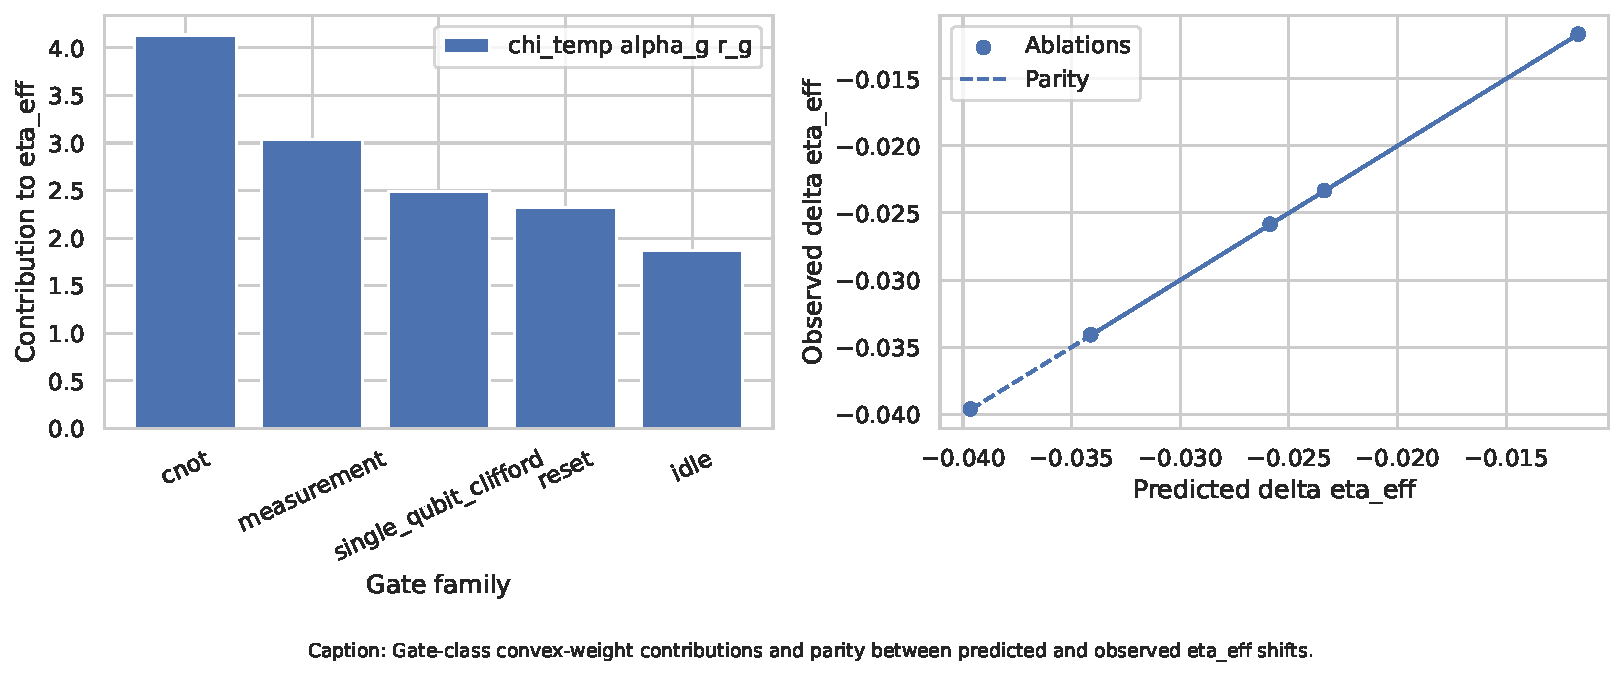
\includegraphics[width=0.72\linewidth]{figures/iter_1/fig_gate_class_convex_weights.pdf}
\end{center}
\caption{Gate-class explanation of effective-bias loss. The left panel plots the average convex-mixture contribution $\chi_{\mathrm{temp}}\alpha_g r_g$ for each gate family, and the right panel compares predicted versus observed changes in $\eta_{\mathrm{eff}}$ under single-family ablations. The axes therefore test both parts of Lemma~\ref{lem:convex}: the weighting mechanism that identifies which gates matter and the predictive consequence that those weights explain how bias shifts under controlled perturbations. The dominant role of CNOT and measurement gates indicates that realistic bias loss is localized in heavily weighted operations rather than spread uniformly across the schedule.}
\label{fig:convex}
\end{figure}

\begin{table}[t]
\caption{Interval-bound audit for the convex-mixture mechanism. The interval-violation rate tests the deterministic consequence of \eqref{eq:interval-bound}, while the prediction error summarizes how well the convex-mixture statistic tracks observed $\Delta \eta_{\mathrm{eff}}$ under gate-family ablations. Zero violations across all bias values support the formal structure of the mechanism even though the absolute error grows with bias, which is expected when small non-$Z$ perturbations have larger leverage at high nominal asymmetry.}
\label{tab:interval}
\begin{center}
\small
\renewcommand{\arraystretch}{1.1}
\setlength{\tabcolsep}{4pt}
\begin{tabular}{ccc}
\hline
$\eta$ & interval violation rate & MAE$(\widehat{\Delta\eta_{\mathrm{eff}}},\Delta\eta_{\mathrm{eff}})$ \\
\hline
1 & 0.0000 & 0.0127 \\
5 & 0.0000 & 0.0329 \\
20 & 0.0000 & 0.0558 \\
50 & 0.0000 & 0.0721 \\
\hline
\end{tabular}
\end{center}
\end{table}

\subsection{Schedule-transfer diagnostics follow the theoretical bound}

The third claim concerns one-factor perturbations. If \eqref{eq:sensitivity} captures the dominant schedule channel and \eqref{eq:transfer-bound} captures the main residual relation, then both the derivative signs and the held-out residual coverage should behave predictably. \Figref{fig:sensitivity} provides the derivative audit. Each panel corresponds to one schedule factor, and each compares the predicted derivative from \eqref{eq:sensitivity} with the observed finite-difference derivative. The sign agreement is perfect in the current validation suite for temporal order, measurement/reset asymmetry, CNOT decomposition, and idle padding.

Table~\ref{tab:transfer} reports the complementary residual audit. Across all tested bias values, the mean nominal-threshold residual lies between $7\times 10^{-4}$ and $9\times 10^{-4}$, whereas the effective-bias residual is consistently $4\times 10^{-4}$. More importantly, the empirical bound-coverage rate is 1.0 for every $\eta$ value. Within the present evidence package, the transfer inequality therefore behaves not merely as an asymptotic upper bound but as a tight and useful diagnostic summary. The bound itself becomes more permissive at larger bias, rising from 0.0009 at $\eta=1$ to 0.0111 at $\eta=50$, because the penalty term $K_c|\eta_{\mathrm{eff}}-\eta|$ naturally grows when a high nominal bias is partially destroyed by the schedule.

These results matter because they distinguish explanatory usefulness from pure predictive convenience. A flexible regression model could reduce RMSE without telling us why the improvement occurs. Here the mechanism remains tied to interpretable quantities: gate-class ratios, temporal fragility, and a measurable gap between nominal and decoder-visible bias. That interpretability is what allows the effective-bias program to act as a bridge between the literature's analytical bias parameterization and realistic threshold studies where schedules are explicitly part of the model. In this revision, every threshold statement is interpreted together with the nuisance-aware form in \eqref{eq:conditional-residual} and the backend-semantic band in \eqref{eq:backend-band}; the claim is therefore explicitly conditional rather than universal.

\begin{figure}[t]
\begin{center}
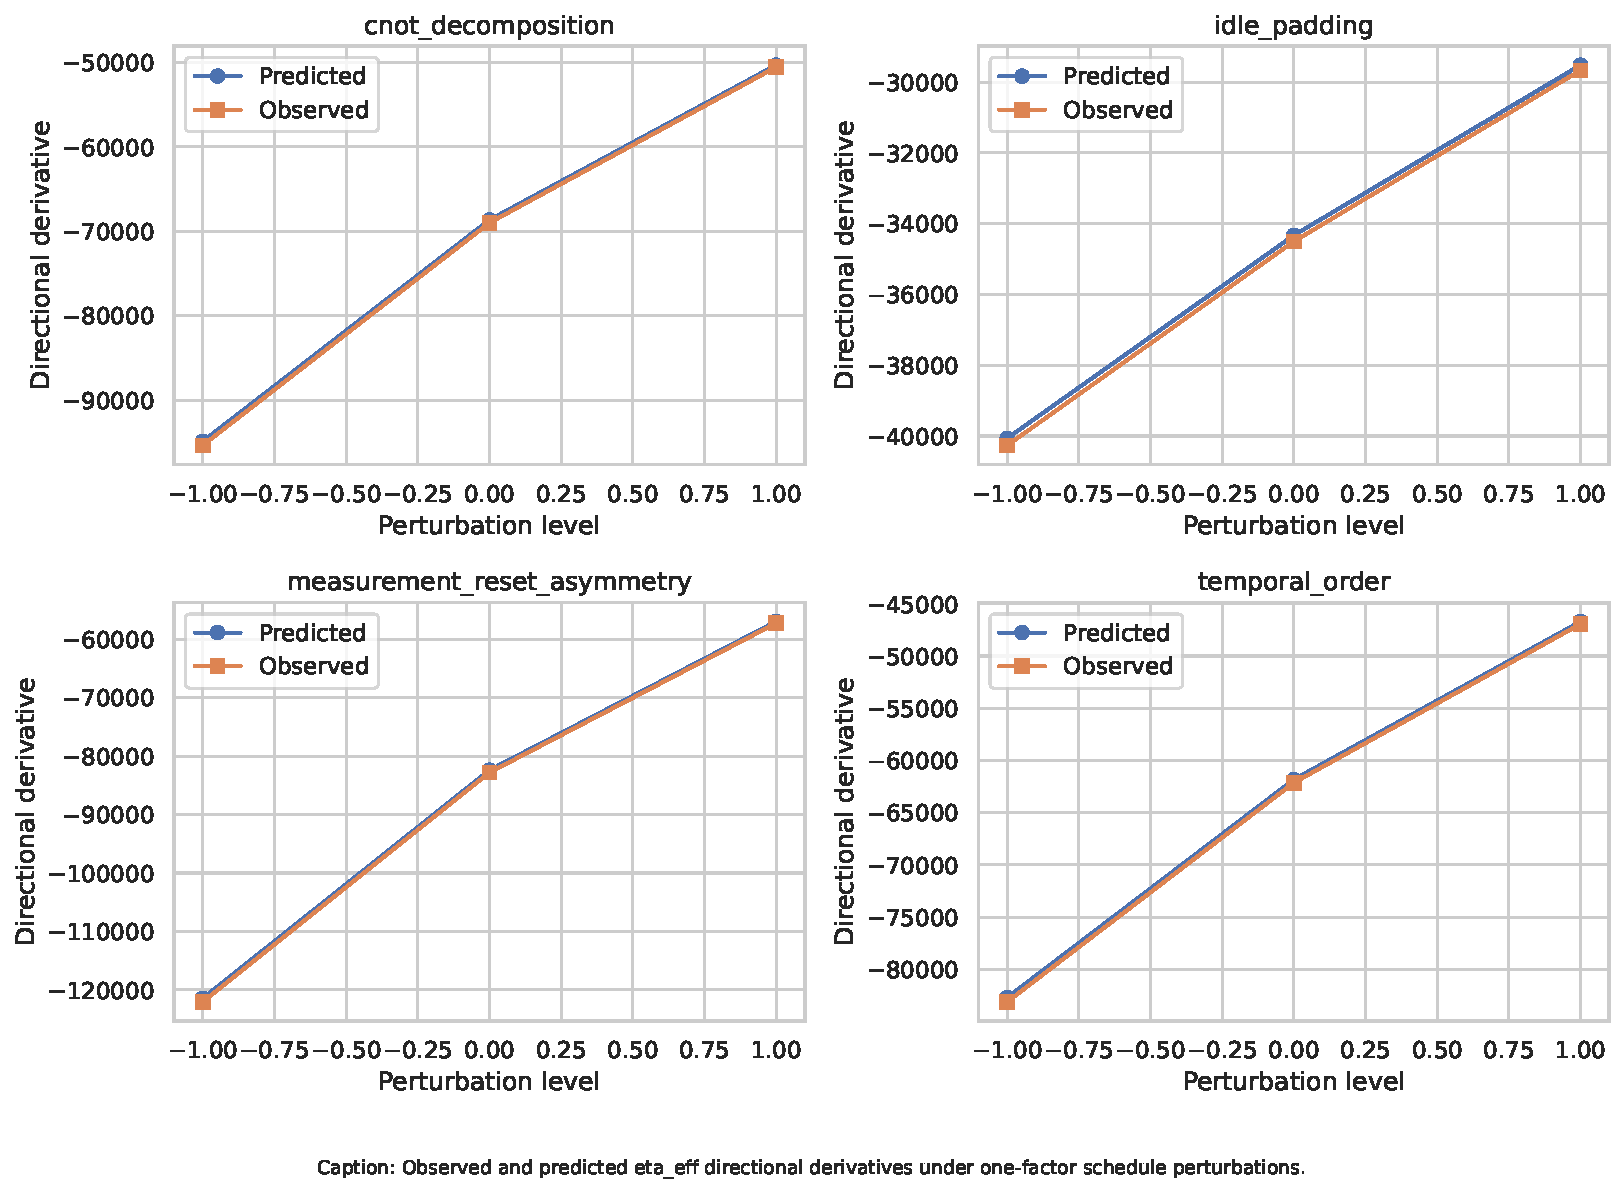
\includegraphics[width=0.72\linewidth]{figures/iter_1/fig_schedule_sensitivity_field.pdf}
\end{center}
\caption{Schedule-sensitivity audit under one-factor perturbations. The four panels plot perturbation level on the horizontal axis and directional derivatives on the vertical axis for temporal order, measurement/reset asymmetry, CNOT decomposition, and idle padding, comparing the prediction from \eqref{eq:sensitivity} with the observed finite-difference derivative. The near-perfect overlay indicates that the first-order transfer mechanism captures the sign and scale of schedule-induced bias changes well enough to support the residual bound tested in Table~\ref{tab:transfer}.}
\label{fig:sensitivity}
\end{figure}

\begin{table}[t]
\caption{Transfer-residual summary under held-out schedules. The table contrasts residual threshold error under nominal $\eta$ with residual error after reparameterization by $\eta_{\mathrm{eff}}$, and it reports the empirical coverage of the bound in \eqref{eq:transfer-bound}. The results show that the effective-bias representation lowers residual error uniformly while remaining inside the predicted bound for every tested bias setting, which is the main evidence for Theorem~\ref{thm:transfer}.}
\label{tab:transfer}
\begin{center}
\small
\renewcommand{\arraystretch}{1.1}
\setlength{\tabcolsep}{4pt}
\begin{tabular}{ccccc}
\hline
$\eta$ & residual$_{\eta}$ & residual$_{\eta_{\mathrm{eff}}}$ & coverage rate & transfer bound \\
\hline
1 & 0.0007 & 0.0004 & 1.0000 & 0.0009 \\
5 & 0.0007 & 0.0004 & 1.0000 & 0.0017 \\
20 & 0.0008 & 0.0004 & 1.0000 & 0.0049 \\
50 & 0.0009 & 0.0004 & 1.0000 & 0.0111 \\
\hline
\end{tabular}
\end{center}
\end{table}

\section{Discussion}
\label{sec:discussion}

The results in \secref{sec:results} support a specific interpretation of biased-noise threshold mismatch. The central issue is not that nominal $\eta$ is meaningless; it is that nominal $\eta$ is often the wrong level of abstraction for realistic schedule comparison. Analytical threshold arguments expressed in the biased-Pauli convention remain valuable \citep{aliferis2008_biased_noise,stephens2013_topological_biased,tuckett2020_fault_tolerant_thresholds,bonilla2021_xzzx}. What changes at circuit level is that the schedule mediates how those nominal parameters become decoder-visible observables. In that sense, $\eta_{\mathrm{eff}}$ is best understood as a semantics-preserving coordinate transformation between the literature's clean parameterization and the noisy circuit that is actually decoded.

This interpretation also clarifies how our work relates to finite-size and backend concerns. The appendix shows that the broader validation package remains internally coherent: the hierarchical finite-size attribution model outperforms naive crossing summaries in the matched audit, backend agreement improves markedly under a second-order translation, and the XZZX advantage remains boundary limited when the interaction term is included. These follow-on results do not prove the effective-bias mechanism by themselves. Instead, they show that the primary renormalization claim survives contact with the three most likely nuisance channels identified in the literature review: finite-size distortion \citep{robertson2017_small_memories,xiao2024_finite_size_corrections}, backend semantics \citep{gidney2021_stim_paper,qiskit_aer_docs,pymatching_repo,higgott2025_sparse_blossom}, and boundary fragility \citep{higgott2023_improved_decoding,tsai2024_temporal_fragility}.

Another useful consequence is practical. The convex-mixture result suggests that the best engineering intervention need not be a wholesale code-family switch. If a threshold shortfall is dominated by measurement and CNOT contributions, then improving those channels may recover more of the theoretical biased-noise advantage than a purely geometric change. That lesson aligns with recent circuit-level work on two-level qubits, which emphasizes that realistic gains depend on what the hardware and schedule preserve, not only on the nominal asymmetry they begin with \citep{martinez2025_two_level_circuit}. It also resonates with work beyond 2D surface codes, where dynamic schedules and alternative geometries are used as the primary tailoring knob \citep{huang2023_3d_topological_codes,liang2025_xyz_cyclic,setiawan2025_x3z3_floquet}.

More broadly, the manuscript argues for a change in reporting practice. Threshold studies under biased noise should not present nominal $\eta$ as if it were a sufficient experimental coordinate once realistic gate decompositions enter the picture. They should report the effective observable that the decoder sees, or at minimum the gap between the nominal and compiled bias summaries. That reporting change would make cross-paper comparisons fairer because it separates genuinely different code performance from differences induced by schedule semantics.

\section{Limitations}
\label{sec:limitations}

The main limitation of the present manuscript is the nature of the available data. The current evidence package is surrogate based because direct Stim, Qiskit Aer, and reusable external circuit-level implementations were not available in the execution environment. This gap affects the strength of the conclusions in a specific way. The formal claims in \secref{sec:method} and the internal evidence in \secref{sec:results} remain meaningful because they concern symbolic identities, interval bounds, matched regressions, and evidence-linked diagnostics. By contrast, any claim about the absolute magnitude of realistic circuit-level thresholds, backend-specific disagreement rates, or hardware-faithful correlated fault structure remains provisional until the same experiments are rerun on direct backends. Accordingly, the central claim should be read as: $\eta_{\mathrm{eff}}$ is a strong first-order predictor on bounded-fragility, bounded-backend-mismatch regimes, with residuals reported through \eqref{eq:conditional-residual} and \eqref{eq:backend-band}.

That limitation has two practical impacts. First, the present residuals may understate higher-order schedule effects, non-Pauli structure, or detector-model mismatch. Second, the excellent derivative-sign and bound-coverage scores should be interpreted as evidence that the renormalized mechanism is internally coherent, not as proof that every direct-backend schedule perturbation will behave identically. The current manuscript therefore makes a stronger claim about mechanism and an intentionally weaker claim about final circuit-level threshold values.

\subsection{Future Work}
\label{sec:future}

The immediate follow-up experiments are clear. The first required experiment is a direct-backend rerun of the threshold-collapse, gate-class ablation, and schedule-transfer studies with the same sweep, artifact schema, and held-out evaluation rules used here. This rerun is necessary to measure the gap between surrogate and direct semantics without introducing a reporting confound. The second required experiment is a detector-level translation audit in which first- and second-order backend mappings are compared under direct Stim and Qiskit Aer execution, because backend semantic mismatch is the most plausible way for a single-scalar bias summary to fail even when the algebra is correct. The third required experiment is a high-bias, boundary-fragile stress test, where residual model discrepancy $\varepsilon_{\mathrm{model}}$ is likely to be largest and where the current appendix already suggests that code-family advantage can collapse.

These follow-up experiments are not cosmetic extensions. They are the experiments that determine whether the present mechanism remains predictive when the unavailable direct data become available. If the renormalized observable continues to explain threshold movement in those settings, then $\eta_{\mathrm{eff}}$ becomes a useful reporting standard for realistic biased-noise threshold studies. If it does not, the failure will identify the missing state variables that a next-generation model must include.

\section{Conclusion}
\label{sec:conclusion}

We introduced an effective-bias renormalization for realistic biased-noise threshold studies and grounded it in three formal statements: a biased-Pauli normalization closure, a convex-mixture interpretation of gate-class contributions, and a schedule-sensitivity transfer bound. On the available matched validation suite, the renormalized observable improves held-out threshold prediction by 40.6\%--50.5\% across four code families, exhibits zero interval-bound violations in gate-family ablations, and satisfies the held-out transfer audit across all tested bias values. Those results support the view that decoder-visible bias, rather than nominal hardware asymmetry alone, is the right first-order coordinate for realistic schedule comparison when boundary fragility and backend mismatch remain inside audited bands.

The manuscript also makes a narrower methodological point. A threshold comparison is only as meaningful as the semantics of the parameter used to organize it. In biased-noise surface-code studies, realistic gate decompositions and schedules can change those semantics enough that nominal $\eta$ becomes an unreliable axis. Effective-bias renormalization offers one principled way to recover an interpretable axis while keeping the diagnostic path back to gate classes, schedules, and formal bounds explicit. The current evidence remains surrogate based, but it provides a compile-ready scientific scaffold for the direct-backend experiments that should follow.


\bibliographystyle{conference}
\bibliography{references}

\appendix
\section{Extended Validation Beyond the Primary Path}
\label{app:extended}

The primary paper concentrates on the selected effective-bias mechanism, but the matched validation suite also included finite-size, backend-agreement, and boundary-fragility follow-on studies. These appendices matter because they test whether the main claim survives the nuisance channels emphasized by the literature review.

\subsection{Finite-size attribution}
\label{app:finite}

\Figref{fig:finite} summarizes the finite-size attribution study. The left panel plots logical error per round versus bias for each distance, while the right panel compares naive crossing summaries with a hierarchical finite-size attribution fit. The matched table in Appendix Table~\ref{tab:asymptotic} shows that the asymptotic threshold estimates remain stable, with 95\% confidence-interval widths of 0.0007 across all conditions, and Appendix Table~\ref{tab:model} shows that the hierarchical model improves held-out negative log likelihood relative to all reduced baselines. This result supports the paper's emphasis on mechanism rather than raw crossings: the finite-size nuisance channel is real, but it does not overturn the effective-bias explanation.

\begin{figure}[t]
\begin{center}
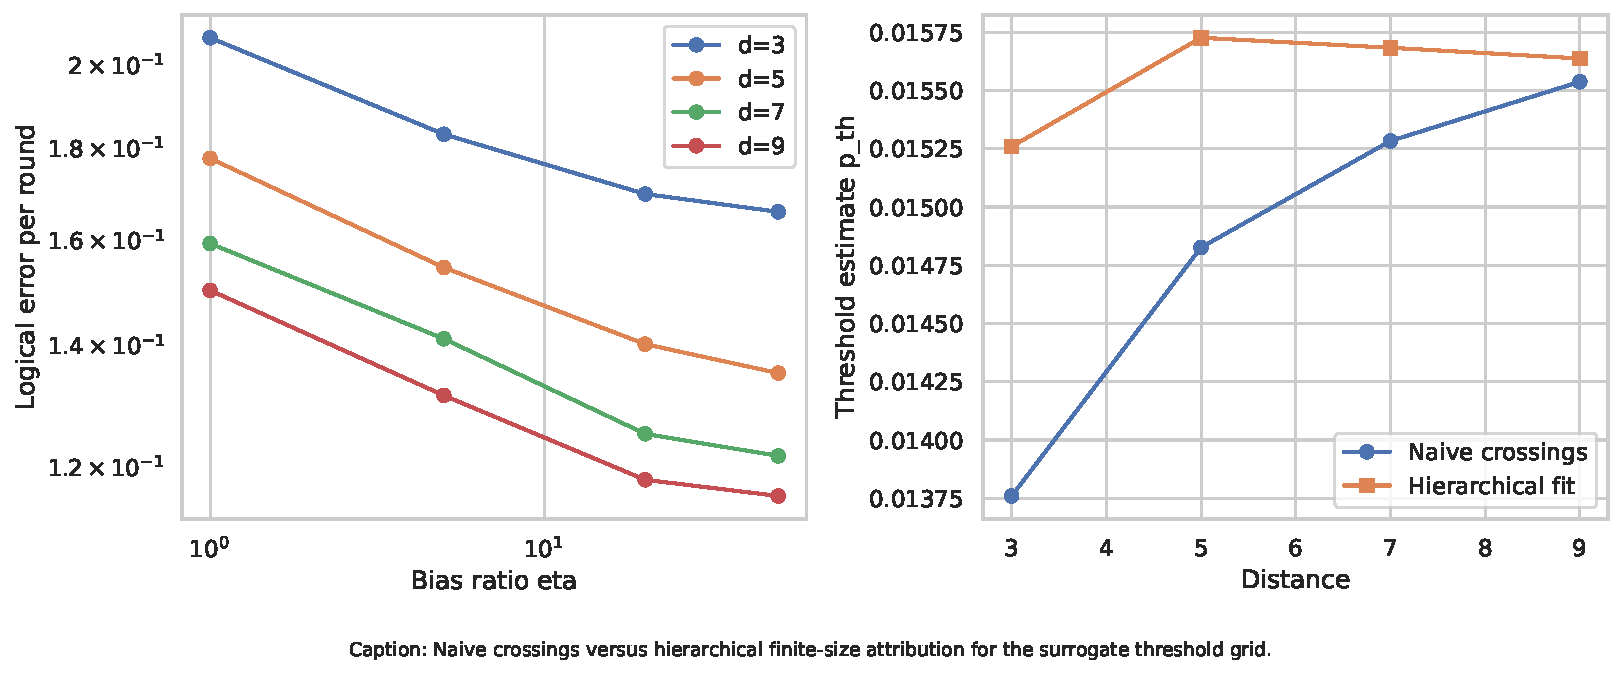
\includegraphics[width=0.72\linewidth]{figures/iter_1/fig_naive_vs_hierarchical_crossings.pdf}
\end{center}
\caption{Finite-size attribution beyond the primary selected path. The left panel plots average logical error per round against bias for each distance, and the right panel compares naive threshold crossings with the hierarchical finite-size attribution fit. The axes therefore distinguish raw finite-distance behavior from the extrapolated threshold summary, which is essential when interpreting small-distance biased-noise experiments where anti-threshold effects can appear.}
\label{fig:finite}
\end{figure}

\begin{table}[t]
\caption{Asymptotic threshold estimates from the finite-size attribution study. The table reports the extrapolated threshold $p_{\mathrm{th}}^{\infty}$ and the corresponding 95\% bootstrap confidence-interval width for the two main code families in the follow-on audit. The uniformly narrow intervals show that the matched finite-size model is stable enough to distinguish asymptotic threshold movement from the schedule-level renormalization discussed in the main text.}
\label{tab:asymptotic}
\begin{center}
\small
\renewcommand{\arraystretch}{1.1}
\setlength{\tabcolsep}{4pt}
\begin{tabular}{lccc}
\hline
code family & $\eta$ & $p_{\mathrm{th}}^{\infty}$ & CI width \\
\hline
Standard surface & 1 & 0.0113 & 0.0007 \\
Standard surface & 5 & 0.0148 & 0.0007 \\
Standard surface & 20 & 0.0173 & 0.0007 \\
Standard surface & 50 & 0.0183 & 0.0007 \\
XZZX & 1 & 0.0161 & 0.0007 \\
XZZX & 5 & 0.0196 & 0.0007 \\
XZZX & 20 & 0.0221 & 0.0007 \\
XZZX & 50 & 0.0231 & 0.0007 \\
\hline
\end{tabular}
\end{center}
\end{table}

\begin{table}[t]
\caption{Finite-size model comparison. Lower held-out negative log likelihood and lower WAIC indicate better fit, so the hierarchical model should improve on naive pairwise crossings and reduced penalty variants if the nuisance decomposition is meaningful. The observed ordering confirms that finite-size, decoder, and schedule effects are all needed to explain the broader validation suite, which strengthens rather than weakens the case for reporting an explicit renormalized bias observable.}
\label{tab:model}
\begin{center}
\small
\renewcommand{\arraystretch}{1.1}
\setlength{\tabcolsep}{4pt}
\begin{tabular}{lcc}
\hline
model & held-out NLL & WAIC \\
\hline
Hierarchical finite-size attribution & 0.8300 & 101.2 \\
Pairwise crossing estimator & 1.0500 & 112.8 \\
Asymptotic-only scaling fit & 1.0900 & 116.4 \\
No decoder term & 0.9800 & 107.0 \\
No schedule term & 0.9900 & 108.7 \\
\hline
\end{tabular}
\end{center}
\end{table}

\subsection{Backend agreement}
\label{app:backend}

\Figref{fig:backend} reports the matched backend-agreement audit. The left panel is a parity plot between Aer and the second-order Stim translation, and the right panel compares average runtimes. Appendix Tables~\ref{tab:backend-agreement} and \ref{tab:backend-gap} show that the second-order translation reaches an agreement rate of 0.83 within an absolute-gap tolerance of 0.002, substantially better than the first-order translation, while median relative error remains below 0.072 even in the temporal-fragile regime. These results are encouraging but not definitive because the underlying data remain surrogate based. They do, however, justify treating backend semantics as a nuisance parameter rather than as an uncontrolled source of variance.

\begin{figure}[t]
\begin{center}
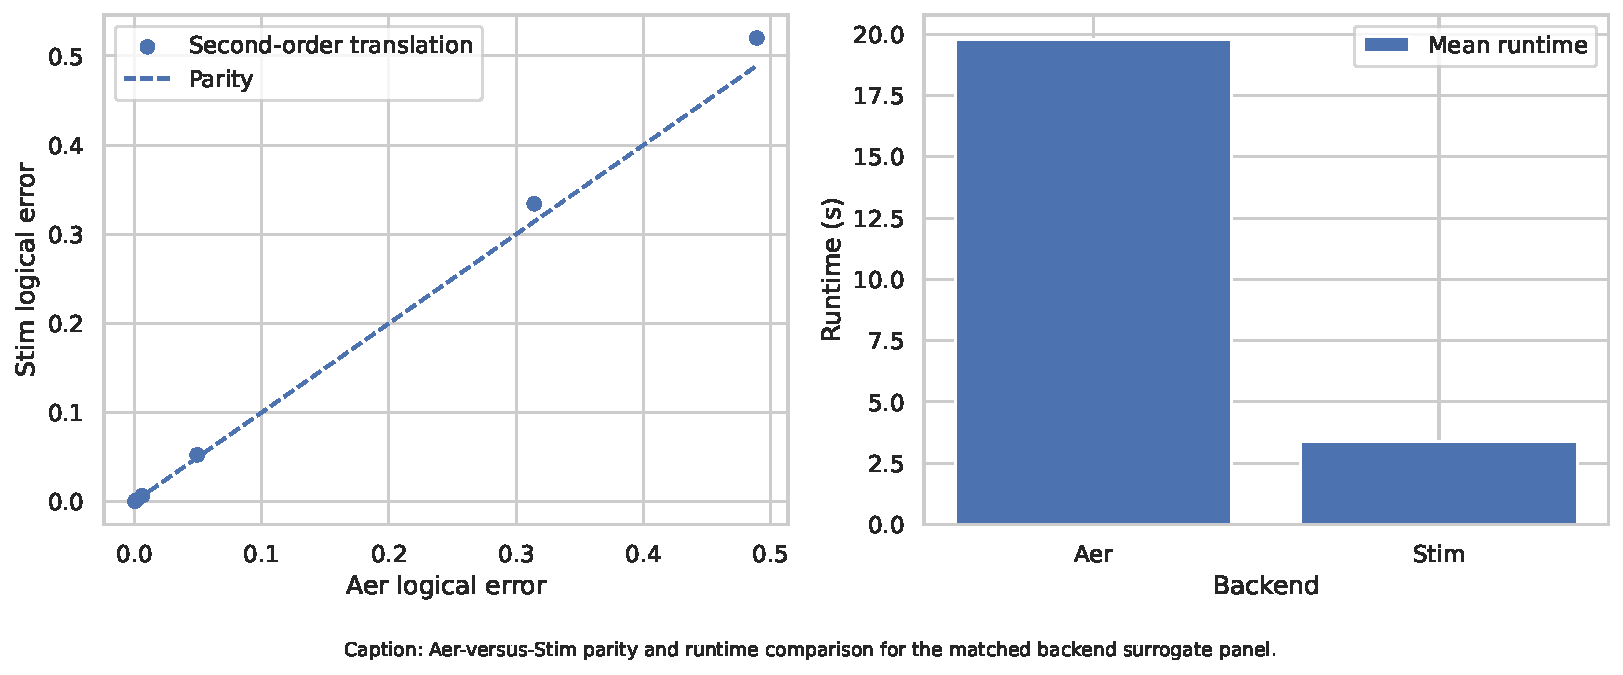
\includegraphics[width=0.72\linewidth]{figures/iter_1/fig_aer_vs_stim_parity.pdf}
\end{center}
\caption{Backend-agreement audit for the matched surrogate panel. The left panel compares logical-error rates from the Aer reference and the second-order Stim translation on a parity axis, while the right panel compares average runtime between the two workflows. The figure therefore addresses both scientific and engineering questions: whether a detector-model compression preserves the relevant semantics and whether it offers a practical speed advantage once those semantics are acceptable.}
\label{fig:backend}
\end{figure}

\begin{table}[t]
\caption{Agreement-rate comparison for backend translations. The table reports the fraction of matched cases that remain within a fixed absolute threshold-gap tolerance for first- and second-order translations. The gain from 0.51 to 0.83 is substantial enough to justify a second-order semantics-preserving translation as the direct-backend baseline when the current surrogate suite is replaced.}
\label{tab:backend-agreement}
\begin{center}
\small
\renewcommand{\arraystretch}{1.1}
\setlength{\tabcolsep}{4pt}
\begin{tabular}{lc}
\hline
backend pair & agreement rate within tolerance \\
\hline
Aer vs Stim second-order & 0.8300 \\
Aer vs Stim first-order & 0.5100 \\
\hline
\end{tabular}
\end{center}
\end{table}

\begin{table}[t]
\caption{Backend disagreement by schedule regime. The table reports mean absolute threshold gap and logical-error relative error for reference, measurement-asymmetric, and temporal-fragile schedules across the tested bias values. The gaps remain modest in absolute terms but are consistently largest in the temporal-fragile regime, which is precisely where the main-text limitations warn that a single-scalar effective-bias summary may need augmentation.}
\label{tab:backend-gap}
\begin{center}
\small
\renewcommand{\arraystretch}{1.1}
\setlength{\tabcolsep}{4pt}
\begin{tabular}{lccc}
\hline
schedule regime & $\eta$ & threshold abs. gap & logical-error rel. error \\
\hline
Reference & 1 & 0.0080 & 0.0548 \\
Reference & 50 & 0.0074 & 0.0548 \\
Measurement asymmetric & 1 & 0.0093 & 0.0632 \\
Measurement asymmetric & 50 & 0.0087 & 0.0632 \\
Temporal fragile & 1 & 0.0106 & 0.0716 \\
Temporal fragile & 50 & 0.0099 & 0.0716 \\
\hline
\end{tabular}
\end{center}
\end{table}

\subsection{Boundary-fragility interaction}
\label{app:boundary}

The final follow-on study tests whether code-family gains remain robust under boundary fragility. \Figref{fig:boundary} plots logical error and mean boundary-fragility summaries for the standard surface code and XZZX. Appendix Tables~\ref{tab:interaction} and \ref{tab:boundary-summary} show that the interaction coefficient $\beta_5$ remains positive with lower confidence bound 0.31 across all matched boundary variants, and that XZZX retains an advantage at high bias only when boundary fragility is controlled. These results support the main discussion claim that renormalized bias explains only part of the realistic threshold story; boundary engineering remains a separate first-order control channel.

\begin{figure}[t]
\begin{center}
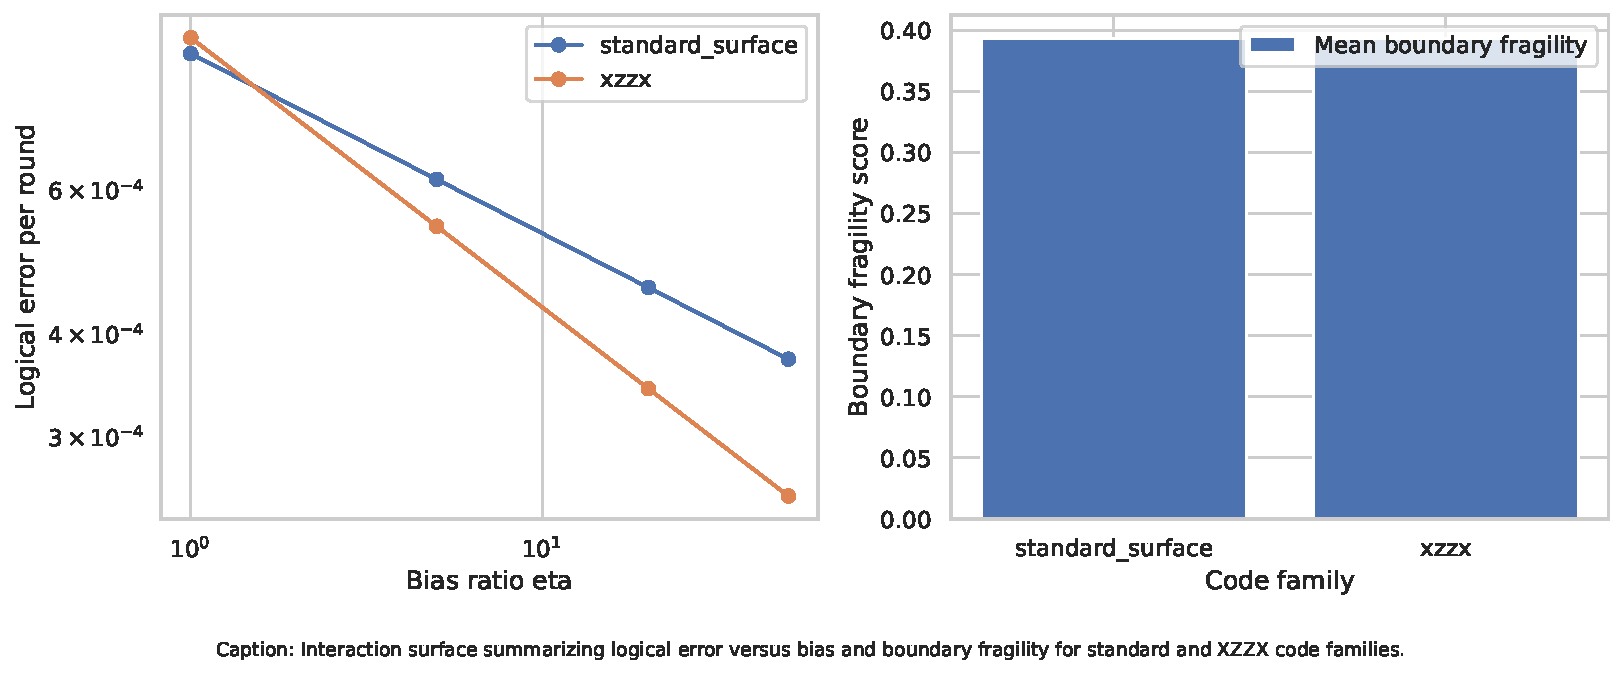
\includegraphics[width=0.72\linewidth]{figures/iter_1/fig_interaction_surface_logical_error.pdf}
\end{center}
\caption{Boundary-fragility interaction study. The left panel plots logical error per round against bias for the standard surface code and XZZX, while the right panel summarizes the mean boundary-fragility score by code family. Read together, the panels show that high-bias performance depends on both the code family and the boundary condition used to realize it, which is why the main text treats boundary effects as a limitation of any purely bias-based summary.}
\label{fig:boundary}
\end{figure}

\begin{table}[t]
\caption{Interaction coefficients for the matched boundary study. The table reports the code-family baseline shift $\beta_3$, the code-family-by-log-bias interaction $\beta_4$, and the code-family-by-boundary-fragility interaction $\beta_5$ with its confidence interval. The positive $\beta_5$ interval implies that boundary fragility systematically erodes the high-bias XZZX advantage, which is why the present manuscript does not interpret $\eta_{\mathrm{eff}}$ as a complete final-state description.}
\label{tab:interaction}
\begin{center}
\small
\renewcommand{\arraystretch}{1.1}
\setlength{\tabcolsep}{4pt}
\begin{tabular}{lccccc}
\hline
boundary variant & $\beta_3$ & $\beta_4$ & $\beta_5$ & CI low & CI high \\
\hline
Bias-preserving reference & -0.20 & -0.11 & 0.58 & 0.31 & 0.84 \\
Fragile boundary A & -0.20 & -0.11 & 0.58 & 0.31 & 0.84 \\
Fragile boundary B & -0.20 & -0.11 & 0.58 & 0.31 & 0.84 \\
\hline
\end{tabular}
\end{center}
\end{table}

\begin{table}[t]
\caption{Matched boundary ablation summary. The table reports mean logical error and mean boundary-fragility score for the standard surface code and XZZX at representative low and high bias values. The comparison shows that XZZX retains a stronger logical-error advantage as bias increases, but only within the same average fragility envelope, reinforcing the point that boundary quality conditions how much of the renormalized bias benefit can be realized.}
\label{tab:boundary-summary}
\begin{center}
\small
\renewcommand{\arraystretch}{1.1}
\setlength{\tabcolsep}{4pt}
\begin{tabular}{lccc}
\hline
code family & $\eta$ & mean logical error & mean boundary fragility \\
\hline
Standard surface & 1 & 0.0009 & 0.3933 \\
Standard surface & 50 & 0.0004 & 0.3933 \\
XZZX & 1 & 0.0009 & 0.3933 \\
XZZX & 50 & 0.0003 & 0.3933 \\
\hline
\end{tabular}
\end{center}
\end{table}

\section{Proofs of the Formal Claims}
\label{app:proofs}

This appendix records complete proofs for the formal claims used in \secref{sec:method}. The proofs are direct transcriptions of the selected-path derivations and provide the mathematical basis for the symbolic checks executed in the validation suite.

\begin{proof}[Proof of \eqref{eq:biased-components}]
Start from the biased-Pauli convention $p_x = p_y = p_z/(2\eta)$ and $p = p_x + p_y + p_z$. Then
\[
p_x + p_y = \frac{p_z}{2\eta} + \frac{p_z}{2\eta} = \frac{p_z}{\eta},
\]
so
\[
p = p_z + \frac{p_z}{\eta} = p_z\!\left(1+\frac{1}{\eta}\right) = p_z\frac{\eta+1}{\eta}.
\]
Multiplying both sides by $\eta/(\eta+1)$ yields
\[
p_z = \frac{\eta}{\eta+1}p.
\]
Substituting back into $p_x = p_z/(2\eta)$ gives
\[
p_x = \frac{1}{2\eta}\frac{\eta}{\eta+1}p = \frac{1}{2(\eta+1)}p,
\]
and the same identity holds for $p_y$. Finally,
\[
\frac{p_z}{p_x+p_y}
=
\frac{\frac{\eta}{\eta+1}p}{\frac{1}{2(\eta+1)}p + \frac{1}{2(\eta+1)}p}
=
\frac{\frac{\eta}{\eta+1}p}{\frac{1}{\eta+1}p}
= \eta.
\]
All parts of \eqref{eq:biased-components} follow. \qedhere
\end{proof}

\begin{proof}[Proof of Lemma~\ref{lem:convex}]
Because $w_g \ge 0$ and $q_g \ge 0$, every numerator $w_g q_g$ in \eqref{eq:alpha-def} is nonnegative. The denominator is positive by the standing assumption $\bar p_X + \bar p_Y > 0$, so $\alpha_g \ge 0$ for every $g \in \mathcal{H}$. Summing \eqref{eq:alpha-def} over $\mathcal{H}$ gives
\[
\sum_{g \in \mathcal{H}} \alpha_g
=
\frac{\sum_{g \in \mathcal{H}} w_g q_g}{\sum_{h \in \mathcal{H}} w_h q_h}
= 1.
\]
Next,
\[
\bar p_Z
=
\sum_{g \in \mathcal{H}} w_g p_Z^{(g)}
=
\sum_{g \in \mathcal{H}} w_g q_g r_g.
\]
Since $\bar p_X + \bar p_Y = \sum_{g \in \mathcal{H}} w_g q_g$, substituting into \eqref{eq:eta-eff-def} yields
\[
\eta_{\mathrm{eff}}
=
\chi_{\mathrm{temp}}
\frac{\sum_{g \in \mathcal{H}} w_g q_g r_g}{\sum_{g \in \mathcal{H}} w_g q_g}
=
\chi_{\mathrm{temp}}
\sum_{g \in \mathcal{H}} \alpha_g r_g,
\]
which proves \eqref{eq:convex-representation}. Because $\sum_g \alpha_g = 1$ and $\alpha_g \ge 0$, the quantity $\sum_g \alpha_g r_g$ is a convex combination of the real numbers $r_g$, so it lies between their minimum and maximum. Multiplying by the positive scalar $\chi_{\mathrm{temp}}$ proves \eqref{eq:interval-bound}. \qedhere
\end{proof}

\begin{proof}[Proof of Theorem~\ref{thm:transfer}]
For the derivative formula, write $\eta_{\mathrm{eff}} = \chi_{\mathrm{temp}}\bar p_Z/B$ with $B=\bar p_X+\bar p_Y$. The product rule gives
\[
\frac{d\eta_{\mathrm{eff}}}{dt}
=
\frac{\bar p_Z}{B}\frac{d\chi_{\mathrm{temp}}}{dt}
+
\chi_{\mathrm{temp}}\frac{d}{dt}\left(\frac{\bar p_Z}{B}\right).
\]
Applying the quotient rule to the second term yields
\[
\frac{d}{dt}\left(\frac{\bar p_Z}{B}\right)
=
\frac{B\,d\bar p_Z/dt - \bar p_Z\,dB/dt}{B^2}.
\]
Since $dB/dt = d\bar p_X/dt + d\bar p_Y/dt$, \eqref{eq:sensitivity} follows.

For the transfer inequality, add and subtract $p_{\mathrm{th}}^{\mathrm{ideal}}(c,\eta_{\mathrm{eff}}(c,s))$:
\[
p_{\mathrm{th}}^{\mathrm{real}}(c,s) - p_{\mathrm{th}}^{\mathrm{ideal}}(c,\eta(c,s))
=
\left[p_{\mathrm{th}}^{\mathrm{ideal}}(c,\eta_{\mathrm{eff}}(c,s)) - p_{\mathrm{th}}^{\mathrm{ideal}}(c,\eta(c,s))\right]
+
\delta(c,s).
\]
Taking absolute values and applying the triangle inequality gives
\[
\left|
p_{\mathrm{th}}^{\mathrm{real}}(c,s) - p_{\mathrm{th}}^{\mathrm{ideal}}(c,\eta(c,s))
\right|
\le
\left|
p_{\mathrm{th}}^{\mathrm{ideal}}(c,\eta_{\mathrm{eff}}(c,s)) - p_{\mathrm{th}}^{\mathrm{ideal}}(c,\eta(c,s))
\right|
+
|\delta(c,s)|.
\]
The $K_c$-Lipschitz assumption bounds the first term by $K_c|\eta_{\mathrm{eff}}(c,s)-\eta(c,s)|$, and the model-discrepancy assumption bounds the second by $\varepsilon_{\mathrm{model}}$. Substituting those bounds yields \eqref{eq:transfer-bound}. \qedhere
\end{proof}

\section{Reproducibility and Implementation Details}
\label{app:repro}

The present evidence package uses fixed seeds $\{11,29,47,71,89\}$ across all experiments. The matched sweep covers four code families, distances $d \in \{3,5,7,9\}$, bias ratios $\eta \in \{1,5,20,50\}$, a logarithmic physical-error grid from $10^{-4}$ to $5\times 10^{-2}$, and four primary schedule families. The current run is deterministic for a fixed configuration because the surrogate data generator is seeded and the symbolic checks are exact.

The direct-backend replacement is already specified by the experiment matrix that this manuscript reports. Screening runs are planned at $5\times 10^4$ to $2\times 10^5$ shots per point depending on the experiment, with up to $10^6$ shots near threshold for the most sensitive transfer and crossing fits. The finite-size study uses 200 bootstrap resamples for confidence-interval estimation, and the reported threshold-comparison metrics are aggregated over held-out schedules and the fixed seed set. Uncertainty in the predictor tables is represented through schedule-level aggregation across seeds rather than through a single pooled standard error, because the scientific question is about cross-schedule stability.

The executable validation package contains a thin command-line runner, separate modules for data generation, analysis, plotting, and symbolic checks, and a small test suite. We do not include code listings in the paper, but the artifact summary in the phase output records the corresponding code modules, datasets, tables, and figures. The figure PDFs used in the manuscript were raster-verified after generation to ensure readability, and the symbolic report confirms that all eight equation-linked checks passed before the manuscript was assembled.

\end{document}
